\documentclass[main.tex]{subfiles}
%
\begin{document}
\chapter{Resultados}
A continuación, se presentan los valores de los parámetros utilizados en todos los resultados siguientes:
\begin{table}[h]
	\centering
	\caption{Par\'ametros Hamiltonianos}
	\begin{tabular}{@{}l|l|l|l|l@{}}
		\toprule
		\textbf{Cavidad}              & \textbf{\begin{tabular}[c]{@{}l@{}}Punto \\ cu\'antico\end{tabular}} & \textbf{\begin{tabular}[c]{@{}l@{}}Bombeo \\ coherente\end{tabular}} & \textbf{\begin{tabular}[c]{@{}l@{}}Interacci\'on\\ electr\'on-fon\'on\end{tabular}} & \textbf{\begin{tabular}[c]{@{}l@{}}Campo\\ magn\'etico\end{tabular}} \\ \midrule
		$\omega_c = 1.00 \text{ meV}$ & $\delta_0 = 40.0 \text{ $\mu$eV}$                                    & $\Omega_1 = 82.0 \text{ $\mu$eV}$                                    & $g_{bb} = 20.0 \text{ $\mu$eV}$                                                     & $g_{hx} = -0.35$                                                     \\
		& $\delta_b = 18.0 \text{ $\mu$eV}$                                    & $\Omega_2 = 0.00 \text{ $\mu$eV}$                                    & $g_{bd} = g_{bb}$                                                                   & $g_{hz} = -2.20$                                                     \\
		& $\delta_d = 5.00 \text{ $\mu$eV}$                                    &                                                                      &                                                                                     & $g_{ex} = -0.65$                                                     \\
		&                                                                      &                                                                      &                                                                                     & $g_{ez} = -0.80$                                                     \\
		&                                                                      &                                                                      &                                                                                     & $\alpha = 20.0 \text{ $\mu$eV/T$^2$}$                                \\
		&                                                                      &                                                                      &                                                                                     & $\mu_B = 57.9 \text{ $\mu$eV/T}$                                     \\ \bottomrule
	\end{tabular}
\end{table}

\begin{table}[h]
	\centering
	\caption{Par\'ametros disipativos}
	\label{tab:my-table}
	\begin{tabular}{@{}l|l@{}}
		\toprule
		\textbf{Cavidad}                & \textbf{\begin{tabular}[c]{@{}l@{}}Punto \\ cu\'antico\end{tabular}} \\ \midrule
		$\kappa = 789 \text{ neV}$ & $\gamma_b = 18.7 \text{ neV}$                                     \\
		& $\gamma_d = 0.1 \gamma_b$                                            \\
		& $\gamma_\phi = 400 \text{ neV}$                                 \\ \bottomrule
	\end{tabular}
\end{table}
\section{Sin campo magn\'etico $(B=0 \text{\normalfont T})$}
En este apartado, se desea mostrar algunos detalles sobre la generación de las gigante-Rabi, tomando como referencia el trabajo realizado por los autores \textcite{Vargas2022}. Primero, se presenta el diagrama de energías, donde se evidencia en qué puntos hay interacción y en cuáles no. En este diagrama, un cruce indica que no hay interacción, mientras que un anticruce señala que sí la hay. Este anticruce también se conoce como desdoblamiento de Rabi. Por lo tanto, se mostrarán los respectivos diagramas de dispersión para evidenciar lo mencionado anteriormente.

\begin{figure}[htbp]
	\centering
	\begin{subfigure}[b]{0.49\textwidth}
		\centering
		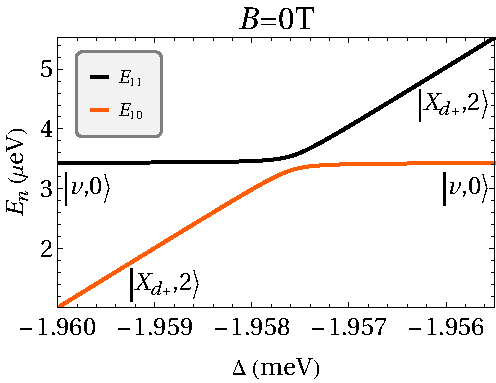
\includegraphics[width=\textwidth]{res/E11E10_B0}
		\caption{Anticruce que evidencia la interacción entre los respectivos estados propios de energía.}
		\label{fig:E11E10_B0}
	\end{subfigure}
	\hfill
	\begin{subfigure}[b]{0.49\textwidth}
		\centering
		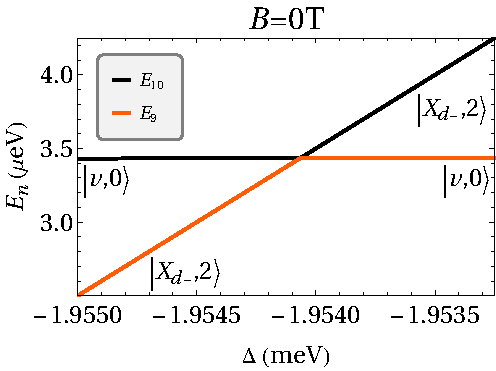
\includegraphics[width=\textwidth]{res/E10E9_B0}
		\caption{Cruce que evidencia la ausencia de interacción entre los respectivos estados propios de energía.}
		\label{fig:E10E9_B0}
	\end{subfigure}
	\begin{subfigure}[b]{0.49\textwidth}
		\centering
		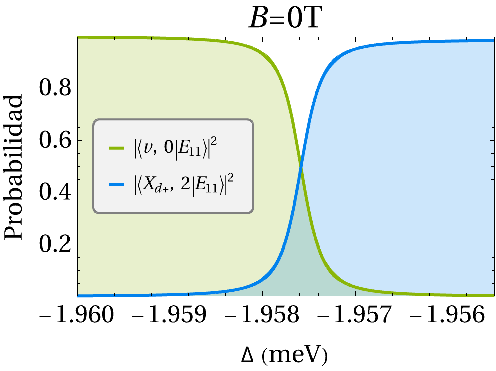
\includegraphics[width=\textwidth]{res/h11_B0}
		\caption{Coeficientes de Hopfield para observar cuáles son los estados de la base involucrados en la interacción.}
		\label{fig:sh11_B0}
	\end{subfigure}
	\hfill
	\begin{subfigure}[b]{0.49\textwidth}
		\centering
		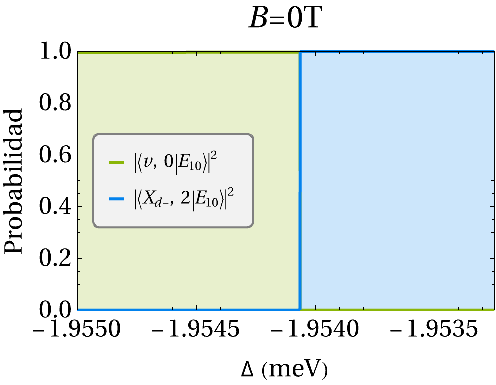
\includegraphics[width=\textwidth]{res/h10_B0}
		\caption{Coeficientes de Hopfield para observar cuáles son los estados de la base involucrados en la reorganización de la base cuando no hay interacción.}
		\label{fig:h10_B0}
	\end{subfigure}
	\begin{subfigure}[b]{0.49\textwidth}
		\centering
		\includegraphics[width=\textwidth]{res/ψ14_B0}
		\caption{Gigante-Rabi entre los estados de la base observados en los coeficientes de Hopfield.}
		\label{fig:ψ14_B0}
	\end{subfigure}
	\hfill
	\begin{subfigure}[b]{0.49\textwidth}
		\centering
		\includegraphics[width=\textwidth]{res/ψ15_B0}
		\caption{La ausencia de la gigante-Rabi, como se esperaba.}
		\label{fig:ψ15_B0}
	\end{subfigure}
	\caption{Aquí observamos dos procesos: a la izquierda, la obtención de la gigante-Rabi a partir del diagrama de dispersión, y a la derecha, cuando no se obtiene la gigante-Rabi.}
	\label{fig:Vladimir}
\end{figure}

Como se observa en la figura \ref{fig:Vladimir}, se detalla el procedimiento numérico para encontrar las gigante-Rabi en general. Aquí se indica que cuando se encuentra un anticruce, se está evidenciando una interacción en la que, en principio, se intercambian los estados de la base entre los respectivos estados propios. Esto se puede comprobar usando los coeficientes de Hopfield, en los que se grafica la probabilidad de cada uno de los estados de la base de alguno de los dos vectores propios involucrados en la interacción. Una vez se obtiene el valor del detuning, $\Delta \approx -n\omega_b$, cuyo valor es negativo debido a que el detuning se define como $\Delta = \omega_b - \omega_L$. Es decir, es negativo porque se está ajustando la energía del láser a un valor mayor que el de la excitación del excitón brillante, condición requerida para generar las gigante-Rabi entre el estado vacío $\ket{v,0}$ y algún estado excitón. Esto indica que el sistema inicialmente se prepara en el estado vacío para que luego evolucione a un estado excitón. La variedad de excitación se entiende en este contexto como el número de excitación del modo fundamental del estado del sistema. El estado vacío tiene una variedad de excitación cero, mientras que el estado $\ket{n,X}$ tiene una variedad de excitación de $n+1$, donde $X$ indica cualquier estado excitón presente en el sistema, ya sean excitones brillantes u oscuros, que pueden ser simétricos o antisimétricos. Cuando la diferencia en la variedad de excitación es mayor a 1, se genera una gigante-Rabi.

\section{Configuraci\'on de Voigt $(\theta = 0^\circ)$}

\section{Configuraci\'on de Faraday $(\theta = 90^\circ)$}

\section{Descomposici\'on espectral}

A continuaci\'on se muestra el espectro de energ\'ias del sistema cuando no hay campo magn\'etico ($B=0$), es decir, el sistema modelado por \parencite{Vargas2022}. Se puede observar en la figura \ref{fig:energia-sin-campo-magnetico} que hay tres transiciones de estado permitidas y una prohibida a diferentes desafinamientos ($\Delta = \omega_b-\omega_L$) con $\omega_b$ siendo la energ\'ia de transici\'on del estado vac\'io ($\ket{v,0}$) al estado excit\'on brillante sim\'etrico ($\ket{X_{b+},0}$) y $\omega_L$ la energ\'ia del l\'aser. A continuaci\'on se muestran las transiciones permitidas con sus desafinamientos correspondientes y la transicion prohibida:
\begin{align}
	\bra{v,0}H\ket{X_{b+},2} &\neq 0 \quad \text{con} \quad \Delta \approx -2.001 \text{ meV},\\
	\bra{v,0}H\ket{X_{b-},2} &\neq 0 \quad \text{con} \quad \Delta \approx -1.981 \text{ meV},\\
	\bra{v,0}H\ket{X_{d+},2} &\neq 0 \quad \text{con} \quad \Delta \approx -1.957 \text{ meV},\\
	\bra{v,0}H\ket{X_{d-},2} &= 0 \quad \forall \;\; \Delta.
\end{align}



Como se puede observar la interacci\'on es del orden de los $\mu$eV obteniendo que la intensidad de la interaccion es la diferencia entre las energias correspondientes. As\'i si se activa el campo magneticos vamos a ver en la figura \ref{fig:detuning-con-campo-magnetico} si el minimo (donde sucede la interaccion entre estados) sufre algun cambio.

\begin{figure}[bh]
	\centering
	\includegraphics[width=.9\linewidth]{../res/det_θ0}
	\caption{Desfinamiento $\Delta$ variando la magnitud del campo magnetico horizontal $\theta=0$ rad, para la gigante-Rabi de cada estado exciton, son cuatro posibles permitidos con diferencia tres entre sus variedades de excitacion, donde se observa que $\Delta$ depende del campo magnetico al cadradado, $\Delta \sim B^2$, con algunas transiciones involucran dependencia lineal del campo magnetico.}
	\label{fig:det_θ0}
\end{figure}

En la figura \ref{fig:detuning-con-campo-magnetico} se observa que el desafinamiento depende de la intensidad campo magnetico horizontal y es diferente para cada una de las transiciones permitidas, ademas, habilita la transicion prohibida anteriormente sin campo magnetico. A continuacion menciono la funcion numerica relacionado con el corrimiento del desafinamiento que me permite producir oscilaciones gigante Rabi con diferencia 3 en las variedades de excitacion:
\begin{align}
	\bra{v,0}H\ket{X_{b+},2} &\quad \text{con} \quad \textcolor{magenta}{\Delta \approx -2.001\text{ meV} - 0.025B - 0.02B^2},\\
	\bra{v,0}H\ket{X_{b-},2} &\quad \text{con} \quad \textcolor{blue}{\Delta \approx -1.981\text{ meV} - 0.01B - 0.02B^2},\\
	\bra{v,0}H\ket{X_{d+},2} &\quad \text{con} \quad \textcolor{darkgreen}{\Delta \approx -1.957\text{ meV} - 0.02B^2},\\
	\bra{v,0}H\ket{X_{d-},2} &\quad \text{con} \quad \textcolor{red}{\Delta \approx -1.954\text{ meV} + 0.018B - 0.02B^2}.
\end{align}


%
\end{document}